\begin{frame}{O comportamento dinâmico em sistema físico}
	\begin{figure}[htb]
		\centering
		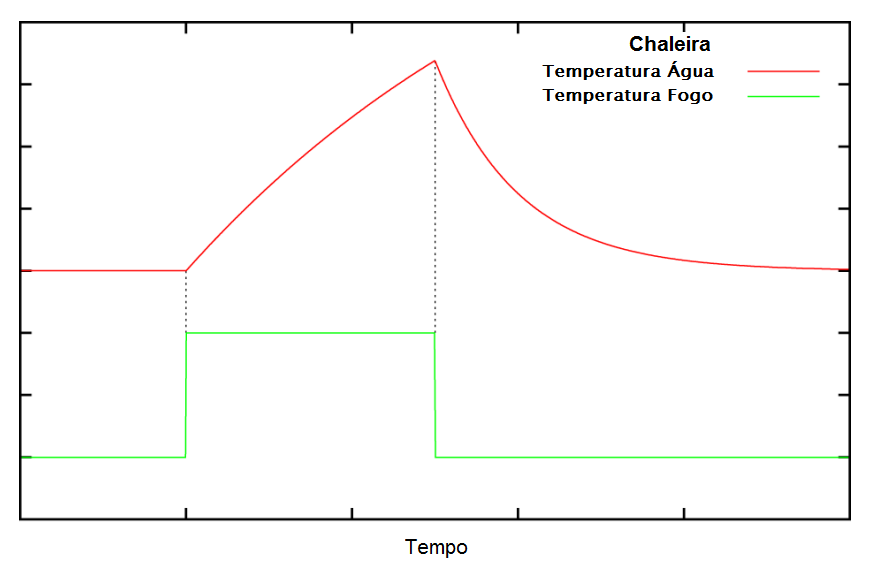
\includegraphics[scale=0.4]{../monograph/images/grafico-chaleira.png}	
		\caption{Dinâmica e comportamento da chaleira aquecendo \cite{Janert2013}}
	\end{figure}
\end{frame}

\begin{frame}{O comportamento dinâmico em sistema físico}
	\begin{figure}[htb]
		\centering
		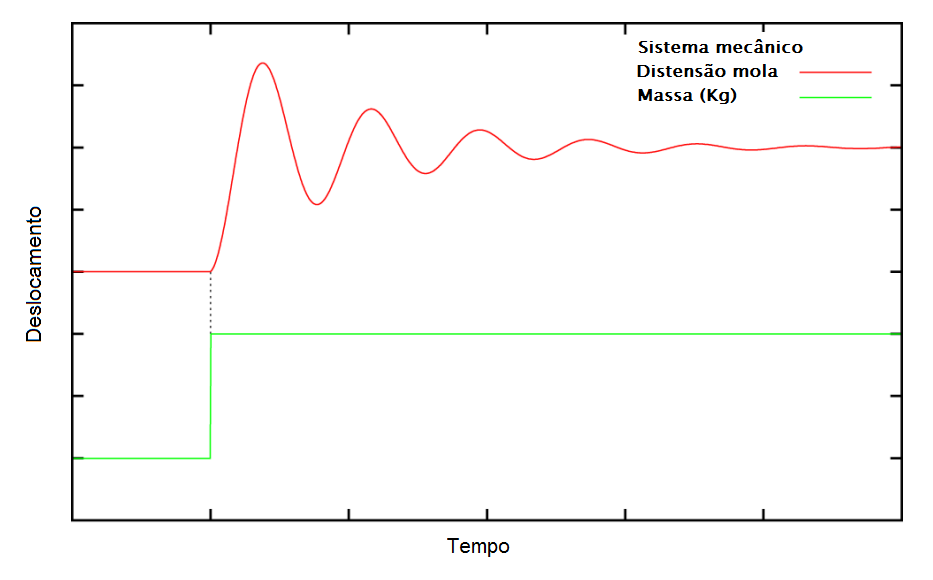
\includegraphics[scale=0.4]{../monograph/images/grafico-mola.png}	
		\caption{Dinâmica e comportamento da mola \cite{Janert2013}}
	\end{figure}
\end{frame}

\begin{frame}{Revisão}
	
	\begin{figure}[!htb]
		\centering 
		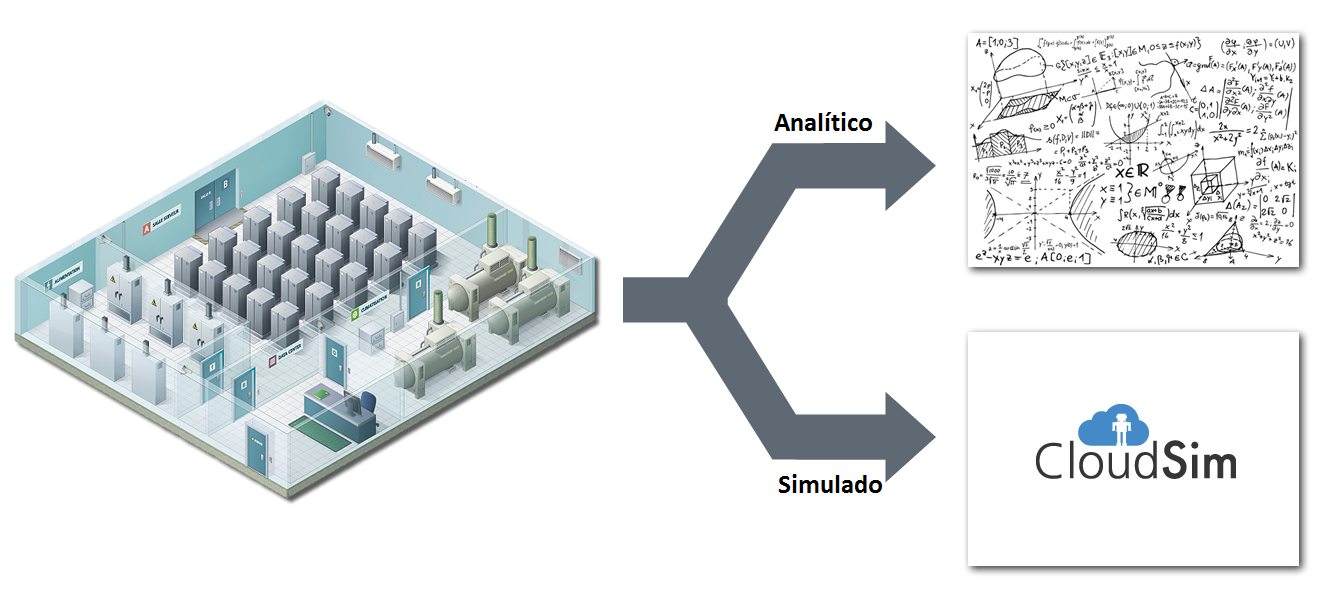
\includegraphics[scale=0.33]{images/abstracao-nobile2.png}
		\caption{Metodologia usada por \cite{Nobile2013}.}
		\label{fig-market-oriented-broker}
	\end{figure}
	
\end{frame}

\begin{frame}{Estratégia Adaptativa}
	
	\begin{figure}
		\center
		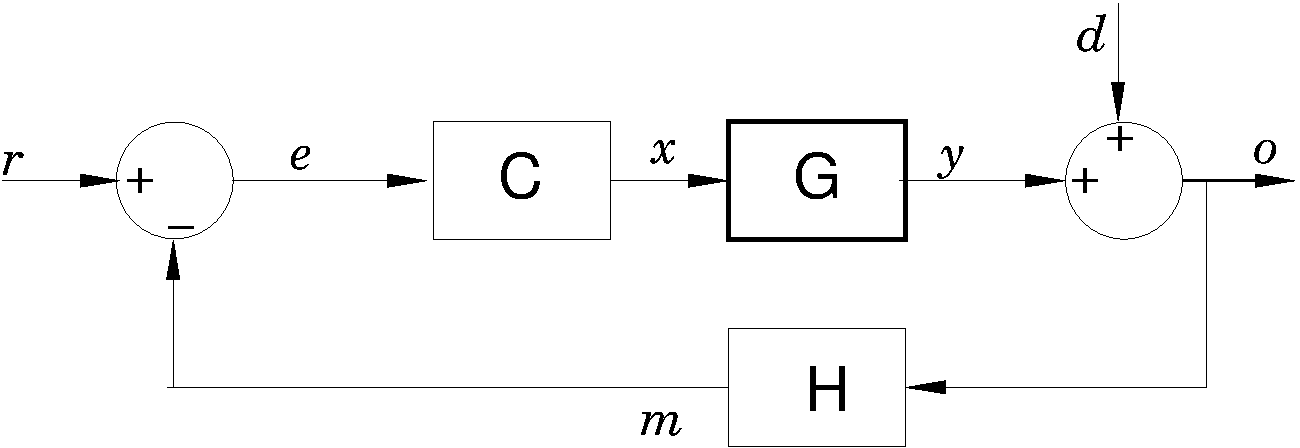
\includegraphics[scale=0.3]{images/feedback-loop-3.pdf}
		\caption{Arquitetura de controle usada por \cite{Nobile2013}.}
		\label{fig:loop-nobile}
	\end{figure}
	
	\begin{itemize}
		\item \textbf{G:} \textit{Datacenter}.
		\item \textbf{H:} Sensor de retroalimentação.
		\item \textbf{C:} Controlador.
		\item \textbf{x:} Número de máquinas virtuais (sinal de controle).
		\item \textbf{o:} Taxa de utilização total (\textbf{y:} taxa relativa).
		\item \textbf{d:} Perturbações (picos de carga, \textit{backups}, etc.) 
		\item \textbf{r:} Entrada de referência da taxa de utilização.
	\end{itemize}
\end{frame}

\begin{frame}{Resultados}
	
	\begin{figure}
		\center
		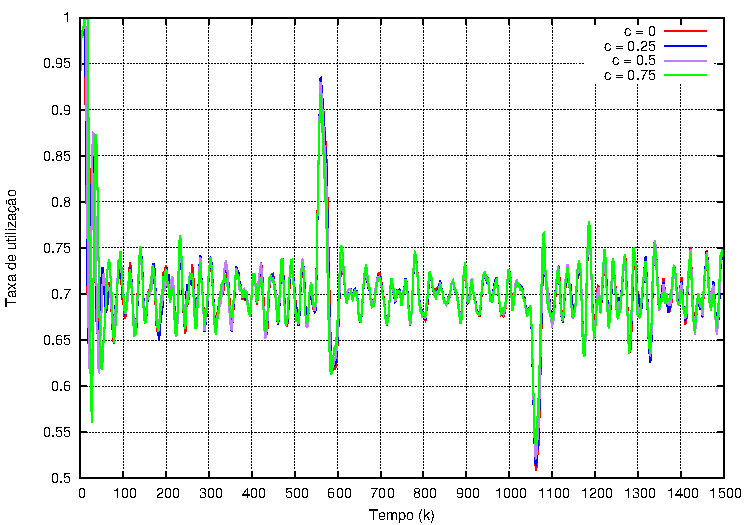
\includegraphics[scale=0.65]{images/resposta-nobile.pdf}
		\caption{Taxa de utilização \cite{Nobile2013}.}
		\label{fig:taxa-nobile}
	\end{figure}
	
\end{frame}

\begin{frame}{Conclusão de \cite{Nobile2013}}
	
	Segundo \cite{Nobile2013}, a \textbf{modelagem das propriedades dinâmicas} e a \textbf{aplicação de técnicas de teoria de controle} em ambientes de recursos elásticos tem impacto apreciável. 
\end{frame}



